\section{Behavior analysis}

In the next table we can see the way the students interacted with the course. Though the differences are not strikingly high, we can observe a behavioral pattern; while \ac{pv} interacted with theory more, \ac{cv} engaged with quizzes more. 

The number may appear small, but \ac{cv} made 7 extra attempts at quizzes in total, while \ac{pv} only 2 despite having more participants. After scaling, that is more than 500\% increase.

\FloatBarrier
\begin{table}[h]
\centering
\renewcommand{\arraystretch}{1.2}
\begin{tabular}{l c c c c c}
\hline
\textbf{Metric} & \textbf{C Mean} & \textbf{C Std} & \textbf{P Mean} & \textbf{P Std} & \textbf{Interpretation} \\
\hline
Quiz interactions & 115.57 & 17.38 & 110.90 & 11.66 & Higher in C \\
Extra theory      & 12.43  & 6.57  & 16.71  & 10.47 & Higher in P \\
Interaction ratio & 0.11   & 0.06  & 0.15   & 0.10  & Higher theory focus in P \\
Extra attempts    & 0.50   & 0.85  & 0.10   & 0.30  & Higher retry behavior in C \\
\hline
\end{tabular}
\caption{Simplified comparison of engagement behavior between Competitive (C) and Playful (P) variants.}
\label{tab:engagement_simple}
\end{table}
\FloatBarrier


Time is difficult to track, since in cases students took breaks with a quiz attempt open, the idle time is included in the calculation as well. However, another pattern can be seen in improvement rates plotted against time spent in the course. While \ac{pv} shows consistent improvement rates across time categories (90-120 minutes contains a single instance, and we view it as an outlier). The final grade in \ac{pv} is also rather consistent.

In the \ac{cv} we can observe a different pattern. Most notably students who had high grades in the intro quiz achieved lower grades in the <60 mins category, while those in the 90-120 and 120+ categories did not experience a drop in performance. That displays a loss of interest and subsequent rushing in some students, which we did not observe in \ac{pv}.

The increased improvement rates in \ac{cv} in 60-90 mins category can be explained by the group having lower intro scores. 

\FloatBarrier
\begin{figure}[ht]
\centering
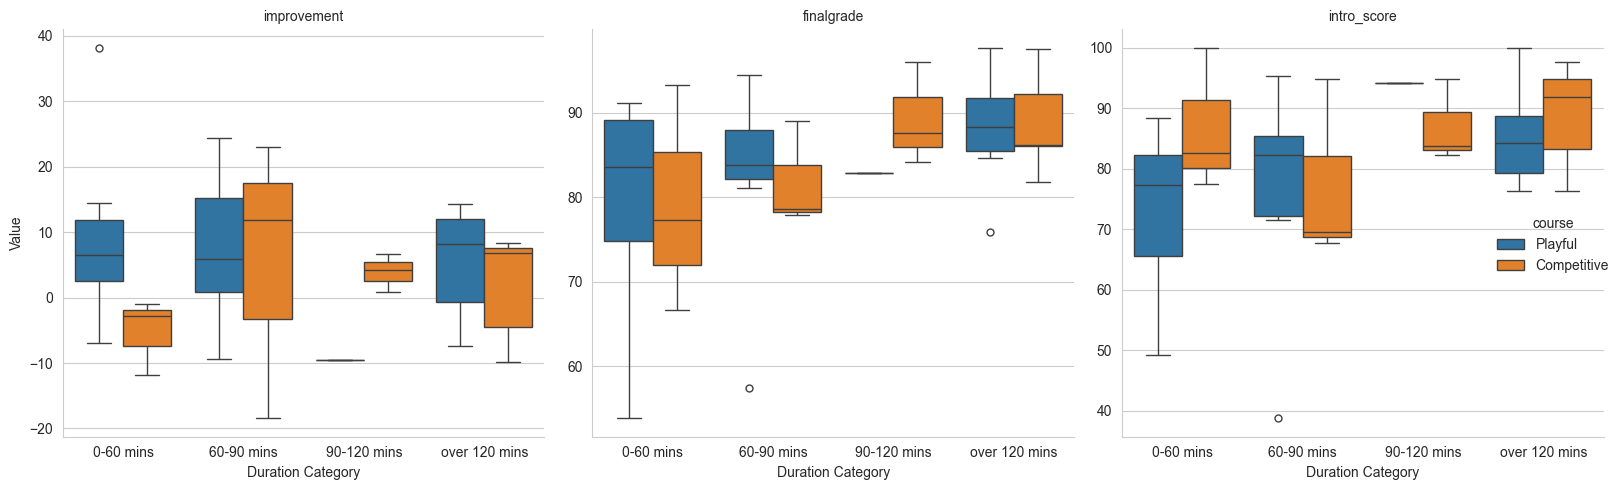
\includegraphics[width=1\textwidth]{assets/images/eval/behavior/improvement_final_intro_by_duration.png}
\caption{Improvement, final grade and intro score by time spent on the course}
\label{fig:improvement_final_intro_by_duration}
\end{figure}
\FloatBarrier

% \textbf{Summary}

% More theory viewing in \ac{pv} is indicative of a more exploratory approach to the study materials, while higher quiz interactions and retries in \ac{cv} shows a more goal-oriented attitude, where students are more prone to accomplishing given activities. There might be an effort to optimize measurable outcomes by retrying quizzes.

% We can again observe a division in \ac{cv}, where a number of students seemed to lose interest during the course, which did not happen in \ac{pv}.

% \todo{we need more support for the retrying. what about remove the fastest category. or check corr again. Or explore other relationships. Or remove claim}